% Note for instructors:
% The R code that is integrated into OpenIntro labs has been highlighted using the R package "highlight", which converts R code to appropriately highlighted latex code. See the end of this document for the original R code (commented out).

\documentclass[11pt]{article}

% Load packages and functions
%%%%%%%%%%%%%%%%
% Header for attribution
%%%%%%%%%%%%%%%%

%\pagestyle{fancy}
%
%\fancyhead{}
%
%\renewcommand{\headrulewidth}{0.25pt}
%\renewcommand{\footrulewidth}{0pt}
%\headsep = 30pt 
%\footskip = 30pt
%
%\chead{{\footnotesize Derivative of \href{http://www.opeintro.org}{\textit{OpenIntro}} project}}

%%%%%%%%%%%%%%%%
% Packages
%%%%%%%%%%%%%%%%

\usepackage[sc]{mathpazo}
%\usepackage[T1]{fontenc}
\usepackage{geometry}
\geometry{verbose,tmargin=2cm,bmargin=2.2cm,lmargin=2.5cm,rmargin=2.5cm}
\setcounter{secnumdepth}{2}
\setcounter{tocdepth}{2}
\usepackage{url}
\usepackage{xcolor}
\usepackage[parfill]{parskip}
\usepackage{graphicx}
\usepackage{amssymb}
\usepackage{amsmath}
\usepackage{epstopdf}
\usepackage{enumerate}
\usepackage{colortbl}
\usepackage{xcolor}
\usepackage{sectsty}
\usepackage{multicol}
\usepackage{fancyhdr}
\usepackage{changepage}
\usepackage{textcomp}
\usepackage{endnotes}
\usepackage{breakurl}

%%%%%%%%%%%%%%%%
% Colors and hyperref
%%%%%%%%%%%%%%%%

\definecolor{oiB}{rgb}{.337,.608,.741}
\definecolor{oiR}{rgb}{.941,.318,.200}
\definecolor{oiG}{rgb}{.298,.447,.114}
\definecolor{oiY}{rgb}{.957,.863,0}

\usepackage[unicode=true, pdfusetitle, bookmarks=true, bookmarksnumbered=true, bookmarksopen=true, bookmarksopenlevel=2, breaklinks=false, pdfborder={0 0 1}, backref=false, colorlinks=true, linkcolor = oiB, urlcolor= oiB]{hyperref}
\hypersetup{pdfstartview={XYZ null null 1}}

%%%%%%%%%%%%%%%%%
%% Color section headings
%%%%%%%%%%%%%%%%%

\allsectionsfont{\color{oiB}}              
 
%%%%%%%%%%%%%%%%
% Exercise environment
%%%%%%%%%%%%%%%%

\newenvironment{exercise}
{
\addvspace{5mm}
\begin{adjustwidth}{0em}{3em}
\begin{itemize}\item[]\refstepcounter{equation}\noindent\normalsize\textbf{\textcolor{oiB}{Exercise \theexercise}}
}
{\normalsize

\addvspace{3mm}
\end{itemize}
\end{adjustwidth}
}

\newcommand\theexercise{\arabic{equation}}

%%%%%%%%%%%%%%%%
% Menu items
%%%%%%%%%%%%%%%%

\newcommand{\menu}[1]{\textsf{#1}}

%%%%%%%%%%%%%%%%
% Formatted url
%%%%%%%%%%%%%%%%

\newcommand{\web}[1]{\urlstyle{same}\textit{\url{#1}}}

%%%%%%%%%%%%%%%%
% Footnote using symbols
% 1 - *
% 2 - dagger
% 3 - double dagger
% 4 - ... 9 (see page 175 of the latex manual)
% http://help-csli.stanford.edu/tex/latex-footnotes.shtml
%%%%%%%%%%%%%%%%

\long\def\symbolfootnote[#1]#2{\begingroup%
\def\thefootnote{\fnsymbol{footnote}}\footnote[#1]{#2}\endgroup}

%%%%%%%%%%%%%%%%
% Non-numbered footnote for license and attribution
%%%%%%%%%%%%%%%%

\newcommand{\license}[1]{\let\thefootnote\relax\footnotetext{#1}}

%%%%%%%%%%%%%%%%
% Set padding in code chunk boxes
%%%%%%%%%%%%%%%%

\setlength\fboxsep{2mm}

%%%%%%%%%%%%%%%%
% Place spacing between text and code chunk boxes
%%%%%%%%%%%%%%%%

\ifdefined\knitrout
  \renewenvironment{knitrout}{
    \vspace{1em}
  }{
    \vspace{1em}
  }
\else
\fi

%%%%%%%%%%%%%%%%
% Redefine inline code commands to change the font to texttt
%%%%%%%%%%%%%%%%

\renewcommand{\hlfunctioncall}[1]{\textcolor[rgb]{0.11,0.53,0.93}{\texttt{#1}}}%

\renewcommand{\hlstring}[1]{\textcolor[rgb]{0.65,0.50,0.39}{\texttt{#1}}}%

\renewcommand{\hlsymbol}[1]{\textcolor[rgb]{0.387,0.581,0.148}{\texttt{#1}}}%

\renewcommand{\hlkeyword}[1]{\textcolor[rgb]{0.31,0.65,0.76}{\texttt{#1}}}%

\renewcommand{\hlargument}[1]{\textcolor[rgb]{0.31,0.41,0.53}{\texttt{#1}}}%

\renewcommand{\hlnumber}[1]{\textcolor[rgb]{0.387,0.581,0.148}{\texttt{#1}}}%



\begin{document}

\section*{Lab 3: Distributions of random variables} % Am I Normal?

\license{This is a product of OpenIntro that is released under a Creative Commons Attribution-NonCommercial-NoDerivs 3.0 Unported (\web{creativecommons.org/licenses/by-nc-nd/3.0/}). This lab was written for OpenIntro by Andrew Bray and Mine \c{C}etinkaya-Rundel.}

In this lab we'll investigate the probability distribution that is most central to statistics: the normal distribution.  If we are confident that our data are nearly normal, that opens the door to many powerful statistical methods.  Here we'll use the graphical tools of R to assess the normality of our data and also learn how to generate random numbers from a normal distribution.

%

\subsection*{The Data}
This week we'll be working with measurements of body dimensions.  This data set contains measurements from 247 men and 260 women, most of whom were considered healthy young adults.

\ttfamily\noindent
\hlfunctioncall{download.file}\hlkeyword{(}\hlstring{"http://www.openintro.org/stat/data/bdims.RData"}\hlkeyword{,}{\ }\hlargument{destfile}{\ }\hlargument{=}{\ }\hlstring{"bdims.RData"}\hlkeyword{)}\hspace*{\fill}\\
\hlstd{}\hlfunctioncall{load}\hlkeyword{(}\hlstring{"bdims.RData"}\hlkeyword{)}\hspace*{\fill}\\
\normalfont

Let's take a quick peek at the first few rows of the data.

\ttfamily\noindent
\hlstd{}\hspace*{\fill}\\
\hlstd{}\hlfunctioncall{head}\hlkeyword{(}\hlsymbol{bdims}\hlkeyword{)}\hspace*{\fill}\\
\normalfont

You'll see that for every observation we have 25 measurements, many of which are either diameters or girths.  A key to the variable names can be found at \web{www.openintro.org/stat/data/bdims.php}, but we'll be focusing on just three columns to get started: weight in kg (\texttt{\hlsymbol{wgt}}), height in cm (\texttt{\hlsymbol{hgt}}), and \texttt{\hlsymbol{sex}} (\texttt{\hlstring{1}} indicates male, \texttt{\hlstring{0}} indicates female).

Since males and females tend to have different body dimensions, it will be useful to create two additional data sets: one with only men and another with only women.

\ttfamily\noindent
\hlstd{}\hspace*{\fill}\\
\hlstd{}\hlsymbol{mdims}{\ }\hlassignement{\usebox{\hlnormalsizeboxlessthan}-}{\ }\hlfunctioncall{subset}\hlkeyword{(}\hlsymbol{bdims}\hlkeyword{,}{\ }\hlsymbol{bdims}\hlkeyword{\usebox{\hlnormalsizeboxdollar}}\hlsymbol{sex}{\ }=={\ }\hlnumber{1}\hlkeyword{)}\hspace*{\fill}\\
\hlstd{}\hlsymbol{fdims}{\ }\hlassignement{\usebox{\hlnormalsizeboxlessthan}-}{\ }\hlfunctioncall{subset}\hlkeyword{(}\hlsymbol{bdims}\hlkeyword{,}{\ }\hlsymbol{bdims}\hlkeyword{\usebox{\hlnormalsizeboxdollar}}\hlsymbol{sex}{\ }=={\ }\hlnumber{0}\hlkeyword{)}\hspace*{\fill}\\
\normalfont

\begin{exercise}
Make a histogram of men's heights and a histogram of women's heights.  How would you compare the various aspects of the two distributions?
\end{exercise}

%

\subsection*{The normal distribution}
In your description of the distributions, did you use words like ``bell-shaped'' or ``normal''?  It's tempting to say so when faced with a unimodal symmetric distribution.

To see how accurate that description is, we can plot a normal distribution curve on top of a histogram to see how closely the data follow a normal distribution. This normal curve should have the same mean and standard deviation as the data. We'll be working with women's heights, so let's store them as a separate object and then calculate some statistics that will be referenced later. 

\ttfamily\noindent
\hlstd{}\hspace*{\fill}\\
\hlstd{}\hlsymbol{fheight}{\ }\hlassignement{\usebox{\hlnormalsizeboxlessthan}-}{\ }\hlsymbol{fdims}\hlkeyword{\usebox{\hlnormalsizeboxdollar}}\hlsymbol{hgt}\hspace*{\fill}\\
\hlstd{}\hlsymbol{fhgtmean}{\ }\hlassignement{\usebox{\hlnormalsizeboxlessthan}-}{\ }\hlfunctioncall{mean}\hlkeyword{(}\hlsymbol{fheight}\hlkeyword{)}\hspace*{\fill}\\
\hlstd{}\hlsymbol{fhgtsd}{\ }{\ }{\ }\hlassignement{\usebox{\hlnormalsizeboxlessthan}-}{\ }\hlfunctioncall{sd}\hlkeyword{(}\hlsymbol{fheight}\hlkeyword{)}\hspace*{\fill}\\
\normalfont

Next we make a density histogram to use as the backdrop and use the \texttt{\hlfunctioncall{lines}} function to overlay a normal probability curve. The difference between a frequency histogram and a density histogram is that while in a frequency histogram the \textit{heights} of the bars add up to the total number of observations, in a density histogram the \textit{areas} of the bars add up to 1. The area of each bar can be calculated as simply the height $\times$ the width of the bar. Using a density histogram allows us to properly overlay a normal distribution curve over the histogram since the curve is a normal probability density function. Frequency and density histograms both display the same exact shape; they only differ in their y-axis. You can verify this by comparing the frequency histogram you constructed earlier and the density histogram created by the commands below.

\ttfamily\noindent
\hlstd{}\hspace*{\fill}\\
\hlstd{}\hlfunctioncall{hist}\hlkeyword{(}\hlsymbol{fheight}\hlkeyword{,}{\ }\hlargument{probability}{\ }\hlargument{=}{\ }\hlnumber{TRUE}\hlkeyword{)}\hspace*{\fill}\\
\hlstd{}\hlsymbol{x}{\ }\hlassignement{\usebox{\hlnormalsizeboxlessthan}-}{\ }\hlnumber{140}\hlkeyword{:}\hlnumber{190}\hspace*{\fill}\\
\hlstd{}\hlsymbol{y}{\ }\hlassignement{\usebox{\hlnormalsizeboxlessthan}-}{\ }\hlfunctioncall{dnorm}\hlkeyword{(}\hlargument{x}{\ }\hlargument{=}{\ }\hlsymbol{x}\hlkeyword{,}{\ }\hlargument{mean}{\ }\hlargument{=}{\ }\hlsymbol{fhgtmean}\hlkeyword{,}{\ }\hlargument{sd}{\ }\hlargument{=}{\ }\hlsymbol{fhgtsd}\hlkeyword{)}\hspace*{\fill}\\
\hlstd{}\hlfunctioncall{lines}\hlkeyword{(}\hlargument{x}{\ }\hlargument{=}{\ }\hlsymbol{x}\hlkeyword{,}{\ }\hlargument{y}{\ }\hlargument{=}{\ }\hlsymbol{y}\hlkeyword{,}{\ }\hlargument{col}{\ }\hlargument{=}{\ }\hlstring{"blue"}\hlkeyword{)}\hspace*{\fill}\\
\normalfont

After plotting the density histogram with the first command, we create the x- and y-coordinates for the normal curve.  We chose the \texttt{\hlsymbol{x}} range as 140 to 190 in order to span the entire range of \texttt{\hlsymbol{fheight}}.  To create \texttt{\hlsymbol{y}}, we use \texttt{\hlfunctioncall{dnorm}} to calculate the density of each of those x-values in a distribution that is normal with mean \texttt{\hlsymbol{fhgtmean}} and standard deviation \texttt{\hlsymbol{fhgtsd}}.  The final command\symbolfootnote[2]{The top of the curve is cut off because the limits of the x- and y-axes are set to best fit the histogram.  To adjust the y-axis you can add a third argument to the histogram function: \texttt{\hlstd{}\hlfunctioncall{hist}\hlkeyword{(}\hlsymbol{fheight}\hlkeyword{,}{\ }\hlargument{probability}{\ }\hlargument{=}{\ }\hlnumber{TRUE}\hlkeyword{,}{\ }{\ }\hlargument{ylim}{\ }\hlargument{=}{\ }\hlfunctioncall{c}\hlkeyword{(}\hlnumber{0}\hlkeyword{,}{\ }\hlnumber{0.06}\hlkeyword{)}\hlkeyword{)}\mbox{}}} draws a curve on the existing plot (the density histogram) by connecting each of the points specified by \texttt{\hlsymbol{x}} and \texttt{\hlsymbol{y}}. The argument \texttt{\hlargument{col}} simply sets the color for the line to be drawn. If we left it out, the line would be drawn in black.

\begin{exercise}
Based on the this plot, does it appear that the data follow a nearly normal distribution?
\end{exercise}

%

\subsection*{Evaluating the normal distribution}
Eyeballing the shape of the histogram is one way to determine if the data appear to be nearly normally distributed, but it can be frustrating to decide just how close the histogram is to the curve. An alternative approach involves constructing a normal probability plot, also called a normal Q-Q plot for ``quantile-quantile''.

\ttfamily\noindent
\hlstd{}\hspace*{\fill}\\
\hlstd{}\hlfunctioncall{qqnorm}\hlkeyword{(}\hlsymbol{fheight}\hlkeyword{)}\hspace*{\fill}\\
\hlstd{}\hlfunctioncall{qqline}\hlkeyword{(}\hlsymbol{fheight}\hlkeyword{)}\hspace*{\fill}\\
\normalfont

A data set that is nearly normal will result in a probability plot where the points closely follow the line.  Any deviations from normality leads to deviations of these points from the line.  The plot for female heights shows points that tend to follow the line but with some errant points towards the tails.  We're left with the same problem that we encountered with the histogram above: how close is close enough?

A useful way to address this question is to rephrase it as: what do probability plots look like for data that I \emph{know} came from a normal distribution?  We can answer this by simulating data from a normal distribution using \texttt{\hlfunctioncall{rnorm}}.

\ttfamily\noindent
\hlstd{}\hspace*{\fill}\\
\hlstd{}\hlsymbol{sim.norm}{\ }\hlassignement{\usebox{\hlnormalsizeboxlessthan}-}{\ }\hlfunctioncall{rnorm}\hlkeyword{(}\hlargument{n}{\ }\hlargument{=}{\ }\hlfunctioncall{length}\hlkeyword{(}\hlsymbol{fheight}\hlkeyword{)}\hlkeyword{,}{\ }\hlargument{mean}{\ }\hlargument{=}{\ }\hlsymbol{fhgtmean}\hlkeyword{,}{\ }\hlargument{sd}{\ }\hlargument{=}{\ }\hlsymbol{fhgtsd}\hlkeyword{)}
\hspace*{\fill}\\
\normalfont

The first argument indicates how many numbers you'd like to generate, which we specify to be the same number of heights in the fdims data set using the \texttt{\hlfunctioncall{length}} function.  The last two arguments determine the mean and standard deviation of the normal distribution from which the simulated sample will be generated.  We can take a look at the shape of our simulated data set, \texttt{\hlsymbol{sim.norm}}, as well as its normal probability plot.

\begin{exercise}
Make a normal probability plot of \texttt{\hlsymbol{sim.norm}}.  Do all of the points fall on the line?  How does this plot compare to the probability plot for the real data?
\end{exercise}

Even better than comparing the original plot to a single plot generated from a normal distribution is to compare it to many more plots using the following function. It may be helpful to click the ``zoom'' button in the plot window.

\ttfamily\noindent
\hlstd{}\hspace*{\fill}\\
\hlstd{}\hlfunctioncall{qqnormsim}\hlkeyword{(}\hlsymbol{fheight}\hlkeyword{)}\hspace*{\fill}\\
\normalfont

\begin{exercise}
Does the normal probability plot for \texttt{fheight} look similar to the plots created for the simulated data?  That is, do plots provide evidence that the female heights are nearly normal?
\end{exercise}

\begin{exercise}
Using the same technique, determine whether or not female weights appear to come from a normal distribution.
\end{exercise}

%

\subsection*{Normal probabilities}
Okay, so now you have a slew of tools to judge whether or not a variable is normally distributed.  Why should we care?

It turns out that statisticians know a lot about the normal distribution.  Once we decide that a random variable is approximately normal, we can answer all sorts of questions about that variable related to probability.  Take, for example, the question of, ``What is the probability that a randomly chosen young adult female is taller than 6 feet (about 182 cm)?"\symbolfootnote[2]{The study that published this data set is clear to point out that the sample was not random and therefore inference to a general population is not suggested.  We do so here only as an exercise.}

If we assume that female heights are normally distributed (a very close approximation is also okay), we can find this probability by calculating a z-score and consulting a z-table.  In R, this is done in one step with the function \texttt{\hlfunctioncall{pnorm}}.

\ttfamily\noindent
\hlstd{}\hspace*{\fill}\\
\hlstd{}\hlnumber{1}{\ }\hlkeyword{-}{\ }\hlfunctioncall{pnorm}\hlkeyword{(}\hlargument{q}{\ }\hlargument{=}{\ }\hlnumber{182}\hlkeyword{,}{\ }\hlargument{mean}{\ }\hlargument{=}{\ }\hlsymbol{fhgtmean}\hlkeyword{,}{\ }\hlargument{sd}{\ }\hlargument{=}{\ }\hlsymbol{fhgtsd}\hlkeyword{)}\hspace*{\fill}\\
\normalfont

Note that the function \texttt{\hlfunctioncall{pnorm}} gives the area under the normal curve below a given value, \texttt{\hlargument{q}}, with a given mean and standard deviation.  Since we're interested in the probability that someone is taller than 6 feet, we have to take one minus that probability.

Assuming a normal distribution has allowed us to calculate a theoretical probability.  If we want to calculate the probability empirically, we simply need to determine how many observations fall above 182 then divide this number by the total sample size.

\ttfamily\noindent
\hlstd{}\hspace*{\fill}\\
\hlstd{}\hlfunctioncall{sum}\hlkeyword{(}\hlsymbol{fheight}{\ }\hlkeyword{\usebox{\hlnormalsizeboxgreaterthan}}{\ }\hlnumber{182}\hlkeyword{)}{\ }\hlkeyword{/}{\ }\hlfunctioncall{length}\hlkeyword{(}\hlsymbol{fheight}\hlkeyword{)}
\hspace*{\fill}\\
\normalfont

Although the probabilities are not exactly the same, they are reasonably close. The closer that your distribution is to being normal, the more accurate the theoretical probabilities will be.

\begin{exercise}
Write out two probability questions that you would like to answer; one regarding female heights and one regarding female weights.  Calculate the those probabilities using both the theoretical normal distribution as well as the empirical distribution (four probabilities in all).  Which variable, height or weight, had a closer agreement between the two methods?
\end{exercise}

\newpage

%

\subsection*{On Your Own}

\begin{enumerate}

\item Now let's consider some of the other variables in the body dimensions data set.  Using the figures on the next page, match the histogram to its normal probability plot.  All of the variables have been standardized (first subtract the mean, then divide by the standard deviation), so the units won't be of any help.  If you are uncertain based on these figures, generate the plots in R to check.

\begin{enumerate}[(a)]

\item The histogram for female biiliac (pelvic) diameter (\texttt{\hlsymbol{bii.di}}) belongs to normal probability plot letter \underline{\makebox[.25in][l]{}}

\item The histogram for female elbow diameter (\texttt{\hlsymbol{elb.di}}) belongs to normal probability plot letter \underline{\makebox[.25in][l]{}}.

\item The histogram for general age (\texttt{\hlsymbol{age}}) belongs to normal probability plot letter \underline{\makebox[.25in][l]{}}.

\item The histogram for female chest depth (\texttt{\hlsymbol{che.de}}) belongs to normal probability plot letter \underline{\makebox[.25in][l]{}}.
\end{enumerate}

\item Note that normal probability plots C and D have a slight stepwise pattern.  Why do you think this is the case?

\item As you can see, normal probably plots can be used both to assess normality and visualize skewness.  Make a normal probability plot for female knee diameter (\texttt{\hlsymbol{kne.di}}).  Based on this normal probability plot, is this variable left skewed, symmetric, or right skewed?  Use a histogram to confirm your findings.

\item What concepts from the textbook are covered in this lab?  What concepts, if any, are not covered in the textbook?  Have you seen these concepts elsewhere, e.g. lecture, discussion section, previous labs, or homework problems?  Be specific in your answer.

\end{enumerate}

\newpage

\begin{figure}[h]
   \centering
	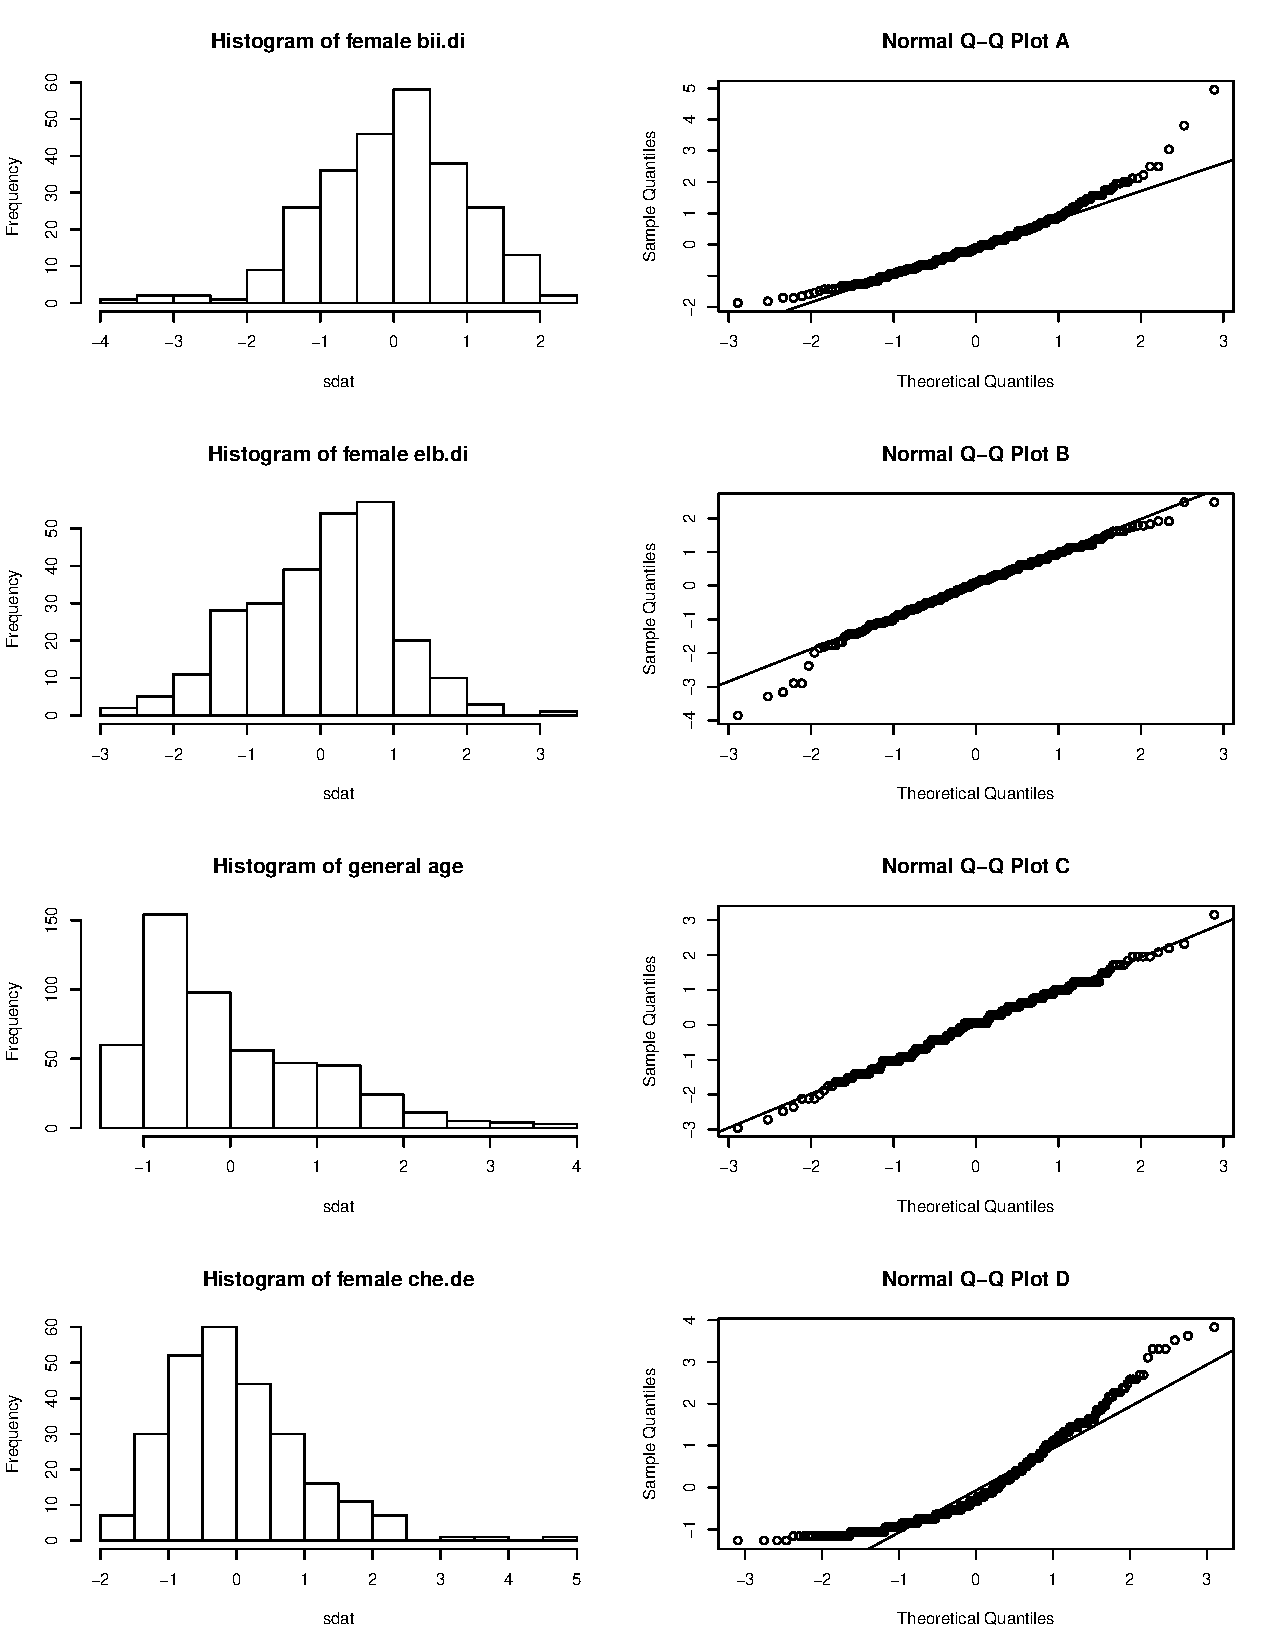
\includegraphics[width=6.25 in]{histQQmatch.pdf}
\end{figure}

\end{document}

%%
% R code:
%%

%% lab code

%download.file("http://www.openintro.org/stat/data/bdims.RData", destfile = "bdims.RData")
%load("bdims.RData")
%
%head(bdims)
%
%mdims <- subset(bdims, bdims$sex == 1)
%fdims <- subset(bdims, bdims$sex == 0)
%
%fheight <- fdims$hgt
%fhgtmean <- mean(fheight)
%fhgtsd   <- sd(fheight)
%
%hist(fheight, probability = TRUE)
%x <- 140:190
%y <- dnorm(x = x, mean = fhgtmean, sd = fhgtsd)
%lines(x = x, y = y, col = "blue")
%
%qqnorm(fheight)
%qqline(fheight)
%
%sim.norm <- rnorm(n = length(fdims$hgt), mean = fhgtmean, sd = fhgtsd)
%
%qqnormsim(fdims$hgt)
%
%1 - pnorm(q = 182, mean = fhgtmean, sd = fhgtsd)
%
%sum(fdims$hgt > 182) / length(fdims$hgt)
%
%# footnote
%hist(fdims$hgt, probability = TRUE,  ylim = c(0, 0.06))

%% highlighting

% highlight("lab3_code.R", renderer = renderer_latex( document = TRUE ) , size = "normalsize", output = "lab3_code_latex")

